\begin{pa} \label{PA:11.2} Let $f(x,y) = 25-x^2-y^2$ on the rectangular domain $R = [-3,3] \times [-4,4]$.

As with partial derivatives, we may treat one of the variables in $f$ as constant and think of the resulting function as a function of a single variable. Now we investigate what happens if we integrate instead of differentiate.

	\ba
	\item  Choose a fixed value of $x$ in the interior of $[-3,3]$. Let
\[A(x) = \int_{-4}^4 f(x,y) \, dy.\]
What is the geometric meaning of the value of $A(x)$ relative to the surface defined by $f$. (Hint: Think about the trace determined by the fixed value of $x$, and consider how $A(x)$ is related to Figure \ref{F:11.2.Cross_section_PA_y}.)
\begin{figure}[ht]
\begin{center}
\begin{minipage}{2.5in}
\begin{center}
%\resizebox{!}{2.4in}{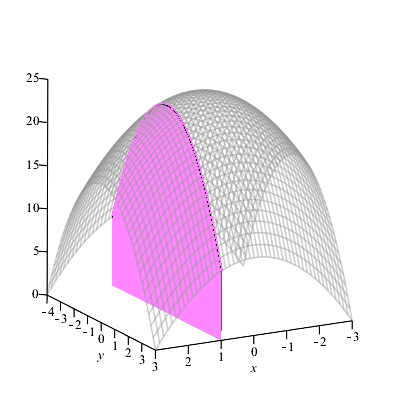
\includegraphics[trim=0cm 0cm 0.25cm 0.5cm,clip]{11_2_Cross_section_PA_y}}
  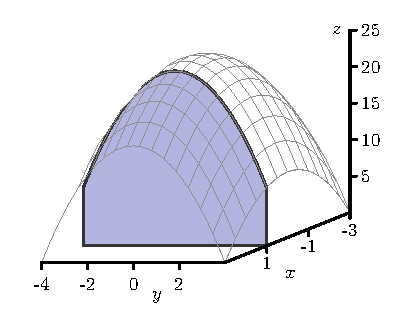
\includegraphics{figures/fig_11_2_preview_slice.eps}
\end{center}
\caption{A cross section with fixed $x$.}
\label{F:11.2.Cross_section_PA_y}
\end{minipage} \hspace{0.2in}
\begin{minipage}{2.5in}
\begin{center}
%\resizebox{!}{2.4in}{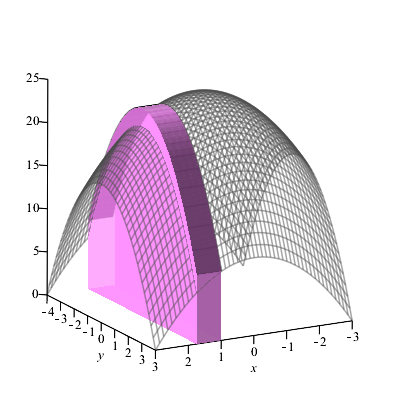
\includegraphics[trim=0cm 0cm 0.25cm 0.5cm,clip]{11_2_Cross_section_PA_y_slab}}
  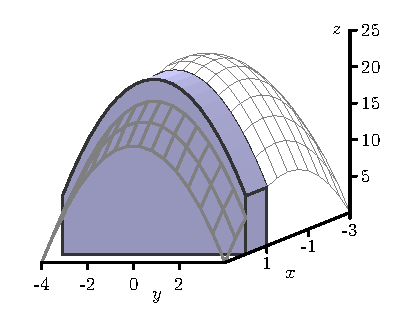
\includegraphics{figures/fig_11_2_preview_thick.eps}
\end{center}
\caption{A cross section with fixed $x$ and $\Delta x$.}
\label{F:11.2.Cross_section_PA_y_slab}
\end{minipage}
\end{center}
\end{figure}
%crop graphics in animate trim=<left> <bottom> <right> <top>, add, clip with \includegraphics



  	\item For a fixed value of $x$, say $x_i^*$, what is the geometric meaning of $A(x_i^*) \ \Delta x$?  (Hint: Consider how $A(x_i^*) \Delta x$ is related to Figure \ref{F:11.2.Cross_section_PA_y_slab}.)


	\item Since $f$ is continuous on $R$, we can define the function $A = A(x)$ at every value of $x$ in $[-3,3]$. Now think about subdividing the $x$-interval $[-3,3]$ into $m$ subintervals, and choosing a value $x_i^*$ in each of those subintervals.  What will be the meaning of the sum $\ds \sum_{i=1}^m A(x_i^*) \ \Delta x$? 


	\item Explain why $\int_{-3}^3 A(x) \, dx$ will determine the exact value of the volume under the surface $z = f(x,y)$ over the rectangle $R$.
%\int_{-3}^3 \left( \int_{-4}^4 f(x,y) \, dy \right) \, dx\]
%The latter integral is an \emph{iterated integral}.


	\ea
\end{pa} 

\begin{activitySolution}
	\ba
	\item  Since $f(x,y) \geq 0$ on the given domain, the value of $A(x)$ tells us the area under the $y$-trace curve for that fixed value of $x$.

  	\item Since $A(x_i^*)$ is an area under the $y$-trace for the value $x = x_i^*$, when we multiply that area by a constant width $\Delta x$, we obtain the volume of a slab obtained by thickening the region under the $x=x_i^*$ trace by a uniform thickness $\Delta x$.


	\item This sum will give us the sum of volumes of slabs with constant cross sections parallel to the $yz$-plane, where the cross sections look like the areas under the graphs of the $x_i^*$ traces. 


	\item As we let $m$ go to infinity, the thickness of the slabs goes to 0 and we are just adding up all of the cross sectional areas of the surface parallel to the $yz$-plane, and so 
\[\int_{-3}^3 A(x) \, dx = \lim_{m \to \infty} \sum_{i=1}^m A(x_i^*) \ \Delta x\]
gives us the volume of the solid under the surface $z = f(x,y)$ over the rectangle $R$.

	\ea

\end{activitySolution}

\afterpa 